\chapter{Sémantiser pour exploiter les données}
Pour pouvoir exploiter les données issues des dépouillements fins, il a été décidé de se baser sur un modèle d'encodage récent qui utilise les technologies du web sémantique. 
\subsubsection*{Les technologies du web sémantique}
Les technologies du web sémantique existent depuis 1997\footnote{\href{https://www.w3.org/2001/sw/wiki/Main\_Page}{https://www.w3.org/2001/sw/wiki/Main\_Page}}, instaurées et maintenues par le W3C elles sont constituées :
\begin{itemize}
    \item Du langage RDF, qui définit une syntaxe pour décrire des entités par des phrases en trois parties sujet/verbe/objet.
    \item Des langages RDFS/OWL qui permettent de produire des modèles de données ou ontologies définissant des catégories d'objets (classes), leurs caractéristiques intrinsèques et les relations qui sont susceptibles de les lier entre elles.
    \item Un langage de requête pour interroger ces données, SPARQL, que nous présenterons plus tard.
\end{itemize}
Ces technologies s'appuient sur l'architecture du Web ; une entité est identifiée par son URI. Pour être plus précis les phrases, appelées triplets, sont composées d'un sujet, d'un prédicat et d'un objet. Un ensemble de triplets est appelé un graphe orienté. 
\par
Les avantages de ces technologies sont, en premier les possibilités que permet la définition des ontologies\footnote{Une ontologie est la définition informatique d'un ensemble de règles et de relations sémantiques pour représenter un modèle de données propre à un domaine identifié.}. Pour peu qu'on les maîtrise, ces technologies permettent de modéliser n'importe quel domaine de connaissances si on est capable de bien identifier les catégories d'entités (classes) qui le composent et les relations nécessaires. Cela permet de gérer la granularité de son modèle de données. Le second avantage porte sur la structure des données ; elles ne sont plus figées dans une arborescence bidimensionnelle, comme elles peuvent l'être dans l'inventaire en EAD. On passe à un graphe multi-dimensionnel. Troisièmement, l'interopérabilité des données est un fondement du web sémantique. En utilisant des URIs pour identifier les entités on peut référencer ces entités et donc établir des relations entre ces entités, y compris des relations d'équivalence. Si par ailleurs on partage les mêmes modèle de référence (ontologies), ou qu'on articule entre eux plusieurs modèles, on pourra plus facilement lier des jeux de données entre eux, échanger des données.

\section{Utilisation de RiC-O}
\subsection{L'arrivée du web sémantique dans les archives}
 Le développement de la science ouverte et de l'open data dans le monde des humanités numériques, lors de la décennie passée, a entraîné un regain d'intérêt pour ces technologies qui ont commencé à être utilisées par différents milieux comme les bibliothèques et les musées. Depuis 2013 un groupe de travail de l'ICA (International Council on Archives) dont fait partie Florence Clavaud, l'EGAD (Expert Group on Archival Description) développe le modèle conceptuel RiC-CM pour représenter les "Records in Contexts", plus clairement pour décrire les documents d'archives dans leurs contextes de création, d'accumulation et d'utilisation au fil du temps. Ce modèle conceptuel fait apparaître quatre entités essentielles : le Record Resource, l'Instantiation\footnote{L'entité Instantiation de RiC représente la manifestation physique d'un Record Resource. Un Record Resource a forcément eu une Instantiation associée lors de sa création mais celle-ci peut avoir été perdue. Les relations associées à l'Instantiation concernent son lieu de conservation, les propriétés physiques du document, son support, les autres manifestations dérivées de l'Instantiation (par exemple une numérisation).}, l'Agent et l'Activity. L'entité Agent est une super entité qui englobe les entités Corporate Bodies, Persons, et Families\footnote{Ces entités existent également dans la norme de description ISAAR(CPF), norme utilisée pour décrire les notices d'autorités archivistiques, relatives aux collectivités, aux personnes et aux familles.}. L'un des enjeux du développement de RiC était de remplacer les quatre standards actuels utilisés dans la description d'archives (et notamment le standard ISAD G, qui a pour norme d'encodage la DTD EAD) par un seul. On peut également souligner l'existence de l'entité Place qui représente un lieu. Vu la part importante d'informations relevées sur les lieux lors des dépouillements (les noms des lieux de passage ou des lieux cités dans l'analyse des actes sous différentes formes, leurs coordonnées, les pays) cette entité sera essentielle pour représenter nos données. Dans une moindre mesure c'est la même chose pour les dates, qui sont représentées par des entités Date dans RiC-CM. Les éléments de datation sont exprimés de trois manières différentes dans les fichiers de dépouillement, sous forme littérale, rédigée et normalisée. Il était donc nécessaire d'avoir ces entités dans le modèle conceptuel afin d'exprimer ces données. La première version de RiC-CM est publiée en août 2016. En février 2021 l'ontologie RiC-O 0.2 est également publiée. Cette ontologie est une transposition technique, en OWL, du modèle conceptuel RiC-CM. C'est l'ontologie de référence pour produire des métadonnées archivistiques en RDF conformes à RiC. La création de cette ontologie nourrit la réflexion sur la logique de RiC-CM. La version 1.0 de RiC-CM et RiC-O doit être publiée à la fin de l'année 2023.

\par
\begin{figure}[ht]
    \centering
    \includegraphics[width=0.8\linewidth]{images/Hiérarchie des classes RiC.png}
    \caption{Tableau hiérarchique des classes du modèle RiC-CM}
    \label{fig:tableauclassericcm}
\end{figure}
\subsection{Un modèle déjà utilisé qui fait ses preuves}
Il s'agit donc d'un modèle encore très récent. Cependant les Archives nationales ont été pionnières dans l'utilisation de RiC, dès 2015. Le Lab a commencé par des expérimentations, puis a lancé plusieurs projets à plus grande échelle, soit directement pour le compte des Archives nationales soit en mettant à disposition son expertise dans des projets extérieurs\footnote{Florence Clavaud.\href{https://rec.unil.ch/videos/florence-clavaud-ric-aux-archives-nationales-de-france-enjeux-realisation-perspectives/}{Records in Contexts (RiC) aux Archives nationales de France : enjeux, réalisations, perspectives. Demi-journée d'information} \textit{RIC (Records in Contexts). Quels changements et quelles perspectives ?}, Association vaudoise des archivistes (AVA), Dec 2022, Lausanne (CH), Suisse. ⟨hal-03957469⟩}. Parmi les projets en cours, soulignons que le Lab a sémantisé tous les référentiels des Archives nationales, avec l'ontologie RiC-O\footnote{\href{https://github.com/ArchivesNationalesFR/Referentiels}{https://github.com/ArchivesNationalesFR/Referentiels}}, en particulier celui des types de document dont nous avons parlé, celui des supports et celui des langues. Ces référentiels ont été facilement intégrés au projet ORESM puisqu'ils suivent le même format que nos données. 
Les membres du groupe EGAD espèrent entraîner une transition vers Records in Context dans tout les services d'archives. Pour aboutir à ce résultat, les Archives nationales réalisent un logiciel nommé RiC-O Converter\footnote{\href{https://github.com/ArchivesNationalesFR/rico-converter}{https://github.com/ArchivesNationalesFR/rico-converter}} qui automatise la transformation des données encodées en EAD et EAC-CPF en données conformes à RiC-O. Ce logiciel a été utilisé pour transformer une partie des descriptions des archives notariales des Archives nationales lors de la réalisation en 2022 d'une plate-forme\footnote{\href{https://sparna-git.github.io/sparnatural-demonstrateur-an/index.html}{https://sparna-git.github.io/sparnatural-demonstrateur-an/index.html}} destinée à tester un éditeur visuel de requêtes SPARQL, Sparnatural, sur lequel nous reviendrons ultérieurement.




\section{Pourquoi étendre l'ontologie ?}
\subsection{Un modèle généraliste, des données spécialisées}
L'ontologie RiC-O comme nous l'avons vue est un modèle qui nous satisfait dans les classes et propriétés qu'il met à notre disposition. Pourtant, pour répondre à la granularité forte de notre gisement de données et pour prendre en compte les spécificités de l'analyse de pièces d'archives médiévales et l'histoire complexe de leur conservation, dans le cadre de ce projet, les relations proposées ne sont pas suffisantes. C'est ce qu'avait déjà estimé Florence Clavaud ; lors de la réalisation de la preuve de concept de 2021, elle avait commencé à lister et modéliser les relations supplémentaires nécessaires pour sémantiser les données de dépouillements. RiC-O par exemple n'a qu'une seule relation pour représenter le lien entre une Instantiation et un Agent qui a conservé ou qui conserve celle-ci, c'est la relation \textbf{has or had holder}\footnote{\href{https://www.ica.org/standards/RiC/ontology\#hasOrHadHolder}{https://www.ica.org/standards/RiC/ontology\#hasOrHadHolder}}. Avec les enjeux fondamentaux du projet, de suivre le parcours des archives et de savoir où et quand elles ont été conservées, il est nécessaire de dépasser cette simple relation qui ne précise pas si la conservation est passée ou actuelle. Même chose pour la relation entre une Instantiation et son Identifier\footnote{La classe Identifier dans RiC-O peut servir à représenter l'ensemble des combinaisons de symboles pour identifier une entité précise, dans notre modèle de données elle fait référence à la cote d'un acte. } \textbf{has or had identifier}\footnote{\href{https://www.ica.org/standards/RiC/ontology\#hasOrHadIdentifier}{https://www.ica.org/standards/RiC/ontology\#hasOrHadIdentifier}}; cette relation peut être utilisée pour relier une archive à sa cote, qu'elle soit actuelle ou passée. Or dans le cadre de notre projet nous avons besoin de distinguer ces deux cas. D'autant plus que la période d'utilisation de la cote est parfois spécifiée dans nos tableaux de dépouillements. Utiliser uniquement ces relations nous aurait fait perdre en précision, ce qui n'était pas envisageable.
\par
Par ailleurs, en ce qui concerne l'analyse diplomatique des documents, pour exprimer la tradition de ces actes nous avons besoin de relations plus précises que celles disponibles dans RiC-O. Pour le chercheur en histoire médiévale, et tout spécialement dans le cadre du projet ORESM, il est important de consigner les liens génétiques reliant les différents états d'un texte ; ceux-ci avaient donc été notés dans les tableaux de dépouillement et il était nécessaire de représenter ces liens avec le même niveau de précision que le spécifiaient ces tableaux. Pour les représenter, on ne peut pas simplement se contenter des relations mises à disposition par RiC-O. Par exemple, la relation \textbf{is copy of}\footnote{\href{https://www.ica.org/standards/RiC/ontology\#isCopyOf}{https://www.ica.org/standards/RiC/ontology\#isCopyOf}}
 permet de relier une copie à son original. Mais comment représenter la relation entre un vidimus et son original ? Même chose pour la relation entre un acte inséré ou un acte extrait, et l'original dont il est issu. Qu'en est-il de la relation de l'Agent aux pièces décrites ? Des notions comme le testateur ou le témoin d'un acte qui sont très importantes dans la période étudiée ne sont pas présentes dans RiC-O 0.2. Ce qui est normal, c'est un modèle qui est conçu avant tout pour être générique. Il offre des solutions pour la description d'archives, afin de répondre aux besoins de la majorité des cas, et surtout donne un cadre pour un étendre le modèle si nécessaire, et en cela il est déjà très utile. Il est évident que le niveau de description des dépouillements effectués dans le cadre du projet ORESM va bien au delà du niveau habituel, davantage encore si on ajoute la spécificité du vocabulaire médiéval. C'est pourquoi cette ontologie a été étendue, pour prendre en compte les relations identifiées comme manquantes et exprimer pleinement le niveau de granularité de notre gisement de données.
 \begin{figure}[!h]
     \centering
     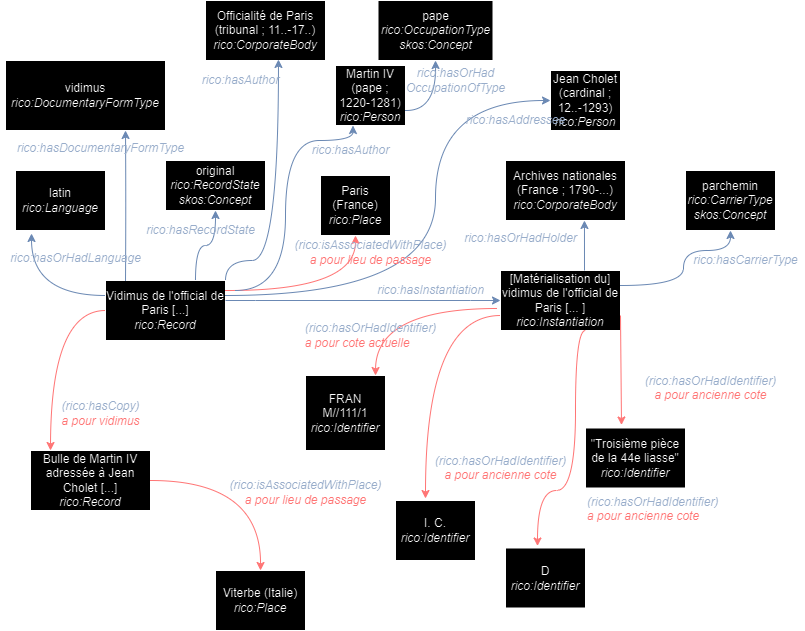
\includegraphics[width=0.8\linewidth]{images/visualisation relations manquantes.png}
     \caption{Visualisation réalisée par Florence Clavaud, pour sa preuve de concept de 2021 qui indique en rouge les relations nécessaires pour le projet ORESM qui n'existent pas dans RiC-O 0.2.}
     \label{fig:enter-label}
 \end{figure}
\subsubsection*{Protégé}
Le logiciel gratuit et open source d'édition d'ontologies Protégé est utilisé dans le cadre de ce projet. Il est développé par l'Université de Stanford. Il permet, avec une interface claire, de visualiser et d'éditer une ontologie. Il est très utilisé par les ingénieurs spécialistes du web sémantique grâce à sa facilité d'accès et l'interface de travail ergonomique qu'il propose. Dans les cas d'ontologies riches et complexes comme RiC-O, il est très utile de pouvoir les ouvrir et les modifier, à l'aide de cet outil, sans devoir impérativement éditer ces ontologies dans leur format source, en l'occurrence XML/RDF. Également en visualisant l'ontologie RiC-O dans Protégé on peut plus facilement appréhender les notions d'héritage. Grâce à cette vue on peut naviguer facilement et comprendre encore mieux les possibilités de RiC-O.
\begin{figure}[ht]
    \centering
    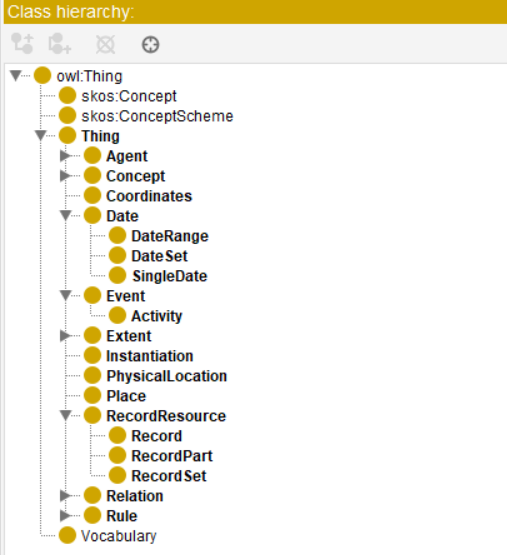
\includegraphics[width=0.6\linewidth]{images/Protégée Classes RiC-O.png}
    \caption{Capture d'écran de la visualisation hiérarchique des classes de l'ontologie RiC-O dans Protégée}
    \label{fig:protegee_classe_rico}
\end{figure}
\subsection{Extension de RiC-O, l'ontologie ORESM}
C'est donc en utilisant Protégé qu'a été élaborée l'ontologie ORESM. Celle-ci reprend l'ensemble des classes et des relations de RiC-O, et lui ajoute de nouvelles relations et une seule classe, dite de relation que nous allons présenter plus loin. Au total 42 nouvelles relations\footnote{Ce nombre prend en compte les relations et leurs inverses.} ont été ajoutées, ainsi que 17 datatype properties\footnote{Une datatype property en OWL est une relation qui lie une entité à une valeur textuelle sans URI. On peut dire que ce sont les attributs de l'entité.} Il a été décidé de libeller et de décrire ces relations en français notamment pour différencier les relations de celles de RiC-O qui sont en anglais, mais également par souci purement pratique : cette ontologie étant centrée sur la description d'archives françaises avec des acteurs français, il n'y avait pas d'intérêt à insérer de l'anglais dans nos travaux. 
\par
Nous évoquions plus haut les relations manquantes pour exprimer le lien entre une institution de conservation et l'Instantiation d'un document, en distinguant une relation passée ou présente. La solution a été de créer deux relations qui sont des sous-propriétés de la relation \textbf{has or had holder}\footnote{\href{https://www.ica.org/standards/RiC/ontology\#hasOrHadHolder}{https://www.ica.org/standards/RiC/ontology\#hasOrHadHolder}}, l'une au passé la relation \textbf{a conservé} et son inverse \textbf{a été conservé par}, et l'autre au présent \textbf{conserve actuellement} et son inverse \textbf{est conservé actuellement par} . Les deux relations inverses sont sous-propriétés de \textbf{'is or was holder of'}\footnote{\href{https://www.ica.org/standards/RiC/ontology\#isOrWasHolderOf}{https://www.ica.org/standards/RiC/ontology\#isOrWasHolderOf}} elle même relation inverse de \textbf{has or had holder}.
\par
Pour ce qui est de la relation entre la cote et une pièce d'archives à laquelle elle se rapporte, deux solutions ont été trouvées. La première comparable au cas des institutions de conservation, a consisté à créer quatre relations d'entité à entité, qui sont des sous-propriétés de \textbf{has or had identifier}\footnote{\href{https://www.ica.org/standards/RiC/ontology\#hasOrHadIdentifier}{https://www.ica.org/standards/RiC/ontology\#hasOrHadIdentifier}} et son inverse. Mais parfois, comme nous l'avons dit, la cote dans le tableau de dépouillement est associée à un élément de datation précis. Or il n'est pas possible, dans une ontologie OWL de qualifier un verbe (une relation). 
\par
Ce que nous voulions avec notre modèle de données, était d'exprimer la relation entre par exemple la cote \textit{BB : I : 13e} et le document coté, en exprimant que cette cote a été utilisée au \textsc{XVIII}\ieme{} siècle. C'est là que les classes de relation fournies par RiC-O sont très intéressantes ; ce sont des classes qui représentent des relations en tant qu'entités. Elles ont les caractéristiques informatiques d'une entité, c'est à dire qu'on peut utiliser des propriétés pour les décrire ; mais elles servent de noeud intermédiaire entre les entités qu'elles relient. C'est pour l'instant la seule classe de relation qui a été ajoutée à l'ontologie. Bien que très utiles, de telles classes doivent être évitées si possible, car bien que l'on gagne en précision, on augmente de manière conséquente le nombre de triplets. Nous envisageons toutefois de créer une classe de relation pour relier le lieu de passage d'un acte et celui-ci, afin d'exprimer la forme littérale d'un lieu par rapport à l'acte dans lequel il apparaît. Ce sera une préoccupation future, une fois que le travail de normalisation des noms de lieu sera fait.
\begin{figure}[h]
    \centering
    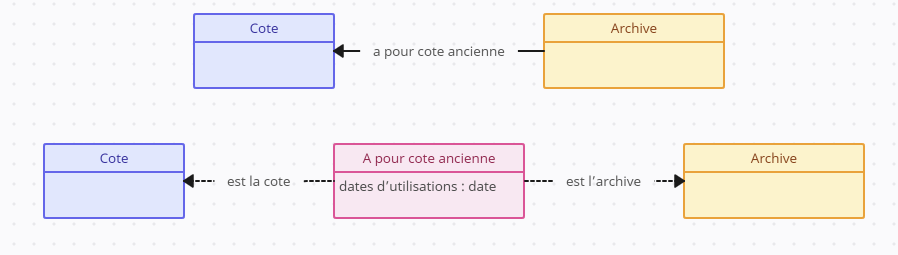
\includegraphics[width=0.9 \linewidth]{images/Classe de relation.png}
    \caption{Représentation UML d'une classe de relation par rapport à une relation simple pour le cas des cotes anciennes.}
    \label{fig:classe_relation}
\end{figure}
\par
Pour résumer nous avons créé une ontologie ORESM en l'articulant avec le cadre générique que constitue RiC-O. Tous les composants que nous avons créés dans cette ontologie sont définis comme des sous-composants RiC-O. Notre modèle est donc en conformité avec l'ontologie qu'il étend, ce qui garantit pour l'avenir l'interopérabilité de nos données avec d'autres jeux de données utilisant RiC-O. Si l'on veut faire rentrer nos données dans un ensemble utilisant RiC-O c'est facilement faisable.  Comme chacune des nouvelles propriétés définies dans l'ontologie ORESM est déclarée comme étant une sous-propriété de RiC-O, un raisonneur connaissant OWL pourra, chaque fois qu'une telle propriété sera instanciée dans nos données, en déduire le triplet utilisant la super-propriété RiC-O. Il sera même ainsi possible, par exemple, au portail FranceArchives\footnote{Le portail FranceArchives a effectué une transition de ses données vers RiC-O en septembre 2023.} d'utiliser les données ORESM si à l'avenir il souhaite les récupérer pour les agréger à celles conformes à RiC-O qu'il utilise déjà ; il lui suffira de n'exploiter que ces triplets conformes à RiC-O, en perdant ainsi, bien sûr, en précision.  Un renvoi vers le futur portail ORESM permettra à l'usager de revenir aux données source.

\section{Construction d'un modèle}
Pour préparer la transformation des données il a été nécessaire d'interroger le contenu des colonnes de nos tableaux de dépouillements. Comme nous l'avons détaillé en quelques exemples précédemment, il fallait faire correspondre une relation ou une entité de notre ontologie avec les données qui ont été dépouillées par l'archiviste, c'est ce qu'on appelle un \textit{data mapping}. Le but principal étant de voir si tout pouvait être exprimé en RDF nous avons, pour chaque colonne, étudié les différentes formes que pouvaient prendre les valeurs et comment les exprimer dans notre ontologie. C'est lors de cette étape que l'ontologie ORESM a été conçue en parallèle, afin de trouver une solution quand RiC-O n'était pas suffisant. Nous avons donc, suivant les conseils de Florence Clavaud, élaboré un \textit{tableau de mapping}\footnote{Ce tableau de mapping est inspiré de la documentation de RiC-O Converter, qui spécifie comment des métadonnées encodées en EAD sont transformées en données RiC-O, disponible sur le github \href{https://github.com/ArchivesNationalesFR/rico-converter/blob/master/docs/EAC_to_Ric-O_0.2_documentation.xlsx}{https://github.com/ArchivesNationalesFR/rico-converter/}. \textit{(Visité le 12/10/2023)}} qui synthétise cette réflexion. C'est un tableau à six colonnes ; chaque ligne représente une colonne des tableaux de dépouillements. On y donne un exemple de valeur que peut prendre une cellule dans ce tableau d'origine, puis on représente comment cette valeur sera exprimée en RDF, on y consigne une remarque si besoin ; une dernière colonne précise, de façon rapide et simple, quelle classe ou datatype property RiC-O est employée. Ce tableau de mapping est en annexe de ce mémoire. \ref{mapping}